\documentclass[a4paper,10pt]{amsart}

\usepackage[protrusion=true,expansion=true]{microtype} 
\usepackage{fancyhdr}
\usepackage[utf8]{inputenc}
\usepackage{graphicx} 
\usepackage{wrapfig} 
\usepackage{enumitem}

\usepackage{mathpazo}
\usepackage[T1]{fontenc}
\usepackage{amsmath}
\usepackage{amssymb}
\usepackage{hyperref}
\usepackage{cleveref}
\usepackage[font=small,labelfont=bf,margin=\parindent,tableposition=top]{caption}
\usepackage{comment}
\usepackage{color}
\usepackage{mathtools}

%%%%%%%%% for quotation
\usepackage{microtype}
\usepackage{times}
\usepackage[english]{babel}
\usepackage{xcolor}
%%%%%%%%%%
% fancy quotes
%%%%%%%%%%
\definecolor{quotemark}{gray}{0.7}
\makeatletter
\def\fquote{%
    \@ifnextchar[{\fquote@i}{\fquote@i[]}%]
           }%
\def\fquote@i[#1]{%
    \def\tempa{#1}%
    \@ifnextchar[{\fquote@ii}{\fquote@ii[]}%]
                 }%
\def\fquote@ii[#1]{%
    \def\tempb{#1}%
    \@ifnextchar[{\fquote@iii}{\fquote@iii[]}%]
                      }%
\def\fquote@iii[#1]{%
    \def\tempc{#1}%
    \vspace{1em}%
    \noindent%
    \begin{list}{}{%
         \setlength{\leftmargin}{0.1\textwidth}%
         \setlength{\rightmargin}{0.1\textwidth}%
                  }%
         \item[]%
         \begin{picture}(0,0)%
         \put(-15,-5){\makebox(0,0){\scalebox{3}{\textcolor{quotemark}{``}}}}%
         \end{picture}%
         \begingroup\itshape}%
 %%%%%%%%%
 \def\endfquote{%
 \endgroup\par%
 \makebox[0pt][l]{%
 \hspace{0.8\textwidth}%
 \begin{picture}(0,0)(0,0)%
 \put(15,15){\makebox(0,0){%
 \scalebox{3}{\color{quotemark}''}}}%
 \end{picture}}%
 \ifx\tempa\empty%
 \else%
    \ifx\tempc\empty%
       \hfill\rule{100pt}{0.5pt}\\\mbox{}\hfill\tempa,\ \emph{\tempb}%
   \else%
       \hfill\rule{100pt}{0.5pt}\\\mbox{}\hfill\tempa,\ \emph{\tempb},\ \tempc%
   \fi\fi\par%
   \vspace{0.5em}%
 \end{list}%
 }%
 \makeatother

\newtheorem{example}{Example}[section]
\newtheorem{theorem}{Theorem}[section]
\newtheorem{proposition}{Proposition}[section]
\newtheorem{corollary}{Corollary}[section]
\newtheorem{definition}{Definition}[section]
\newtheorem{lemma}{Lemma}[section]
\newtheorem{remark}{Remark}[section]
\newtheorem{question}{Question}[section]
\newtheorem{conjecture}{Conjecture}[section]

\newcommand{\AAA}{\mathfrak A}
\newcommand{\BBB}{\mathcal B}
\newcommand{\CCC}{\mathcal C}
\newcommand{\HHH}{\mathcal H} %for Hilbert space
\newcommand{\LLL}{\mathcal L} % for lattice
\newcommand{\MMM}{\mathcal M}
\newcommand{\UUU}{\mathcal U}
\newcommand{\FFF}{\mathcal F}
\newcommand{\A}{\mathcal{A}}
\newcommand{\X}{\mathcal X}
\newcommand{\SSS}{\mathcal S}
\newcommand{\DDD}{\mathfrak D}

\newcommand{\Lat}{\mathcal Lat}
\newcommand{\Alg}{\mathcal Alg}
\newcommand{\tensor}{\mathop{\bar \otimes}}
\newcommand{\tr}{\tau}
\newcommand{\C}{\mathbb C} %for complex number
\newcommand{\R}{\mathbb R}  %for real number
\newcommand{\Z}{\mathbb Z} %for integer
\newcommand{\N}{\mathbb N} % for nature number
\newcommand{\Q}{\mathbb Q} % for rational number

\providecommand{\sceil}[1]{\left \lceil #1 \right \rceil }
\providecommand{\sfloor}[1]{\left \lceil #1 \right \rceil }
\DeclarePairedDelimiter\ceil{\lceil}{\rceil}
\DeclarePairedDelimiter\floor{\lfloor}{\rfloor}
% self defined vars
\newcommand{\titleinfo}{Wei Fei's Note}
\newcommand{\authorinfo}{Wei Fei} 

\linespread{1.05}
\pagestyle{fancyplain}
\fancyhf{}
\fancyhf[HLE,HRO]{\titleinfo}
\fancyhf[HRE,HLO]{\authorinfo}
\fancyhf[FC]{\thepage}

\begin{document}

\title{\LARGE\textbf{\titleinfo}} 

\author{\large\textsc{\authorinfo}} 
\address{AMSS}  
\email{}

\date{}

%\renewcommand{\abstractname}{Summary} 

\begin{abstract}
    Note on Wei Fei's lecture.
\end{abstract}

% Keywords
\subjclass[2010]{Primary 47L75; Secondary 15A30}
\keywords{Number Theory}

\thanks{}

\maketitle

\section{Notations}
Let $\SSS(\R)$ be the Schwartz class, i.e., 
\begin{align*}
    \SSS(\R) = \{f \in C^{\infty}(\R) : 
        sup_{t \in \R}|t^{k}\frac{d^{l}}{dt^{l}}f(t)| < \infty 
    \mbox{ for any $k, l \in \N \cup \{0\}$} \}.
\end{align*}

Let $f \in \SSS(\R)$. The Fourier transform $\Hat{f}$ is
\begin{align*}
    \Hat{f}(s) = \int^{+\infty}_{-\infty} f(t)e^{-2\pi i st}dt, 
    \mbox{ for any $s \in \R$}.
\end{align*}
We have
\begin{align*}
    f(t) =  \int^{+\infty}_{-\infty} \Hat{f}(s)e^{2\pi i ts}ds, 
    \mbox{ for any $t \in \R$}.
\end{align*}


\section{Important formula}

\subsection{Partial Summation Formula}
\begin{lemma}
    Let $f(x) \in C^{1}([a, b])$. Then
    \begin{align*}
        \sum_{a < n \leq b} c_n f(n) = C(b)f(b) - \int^{b}_{a}C(x)f'(x)dx, 
    \end{align*}
    where
    \begin{align*}
        C(x) = \sum_{a < n \leq x} c_n,  \qquad c_n \in \C.
    \end{align*}
\end{lemma}

\begin{theorem}[Possion Summation Formula]
    Let $f$ in $\SSS(\R)$. We have
    \begin{align*}
        \sum_{n \in \Z}f(n) = \sum_{n \in \Z} \Hat{f}(n).
    \end{align*}
    If $f(x) = f(-x)$, then
    \begin{align*}
        \sum^{\infty}_{n=1}f(n) = \sum^{\infty}_{n=1}\Hat{f}(n) +
        \frac{1}{2}(\Hat{f}(0)-f(0)).
    \end{align*}
\end{theorem}

\begin{proof}
    Let 
    \begin{align*}
        g(\theta) = \sum_{n \in \Z}f(\theta+n).
    \end{align*}
    Since $f \in \SSS(\R)$, $g(\theta)$ is a well-defined 
    function of period $1$ such that
    \begin{align*}
        g(\theta) = \sum_{n \in Z} \Hat{f}(n) e^{2\pi i \theta}.  
    \end{align*}
    Let $\theta = 0$, we have
    \begin{align*}
        \sum_{n \in \Z}f(n) = \sum_{n \in \Z} \Hat{f}(n).
    \end{align*}
\end{proof}

\begin{example}
    Let $f(x) = e^{-\pi x^2 y}$.
    \begin{align*}
        \Hat{f}(x)= y^{-\frac{1}{2}}e^{-\frac{\pi x^2}{y}}. 
    \end{align*}
\end{example}

\section{Entire Function}

\begin{lemma}
Let $\{a_{n}\}_{n} \subset \C$ be a sequence, 
\begin{align*}
    0 < |a_{1}| \leq |a_{2}| \leq \cdots \leq |a_{n}| \leq \cdots,
    \mbox{ and } |a_{n}| \rightarrow \infty.
\end{align*}
Then there exists a entire function $f$ such that $f(s) = 0$ if and 
only if $s \in \{a_{n}\}_{n}$.
\end{lemma}

\begin{proof}
   Let 
   \begin{align*}
       h_{n} = (1 - \frac{s}{a_n})e^{\frac{s}{a_{n}}
           +\frac{1}{2}(\frac{s}{a_{n}})^{2} 
            +\frac{1}{3}(\frac{s}{a_{n}})^{3} + \cdots
        +\frac{1}{n}(\frac{s}{a_{n}})^{n}}.
   \end{align*}
   Then
   \begin{align*}
       f(s) = \prod_{n=1}^{\infty}h_{n}(s)   
   \end{align*}
   satisfies the condition.
\end{proof}

\begin{remark}
Let $\{a_{n}\}_{n} \subset \C$ be a sequence, 
\begin{align*}
    0 < |a_{1}| \leq |a_{2}| \leq \cdots \leq |a_{n}| \leq \cdots,
    \mbox{ and } |a_{n}| \rightarrow \infty.
\end{align*}
If $\sum_{n}\frac{1}{|a_{n}|^{p+1}} < \infty$, then we could 
use
\begin{align*}
       h_{n} = (1 - \frac{s}{a_n})e^{\frac{s}{a_{n}}
           +\frac{1}{2}(\frac{s}{a_{n}})^{2} 
            +\frac{1}{3}(\frac{s}{a_{n}})^{3} + \cdots
        +\frac{1}{p}(\frac{s}{a_{n}})^{p}}.
   \end{align*}
in the above proof.
\end{remark}

\begin{example}
    Let $\{n\}_{n \in \Z}$. Then
    \begin{align*}
        f(s) = s\prod_{n \in \N}(1-\frac{s}{n})(1+\frac{s}{n}).  
    \end{align*}
\end{example}

\begin{lemma}
Let $\{a_{n}\}_{n} \subset \C$ be a sequence, 
\begin{align*}
    0 < |a_{1}| \leq |a_{2}| \leq \cdots \leq |a_{n}| \leq \cdots,
    \mbox{ and } |a_{n}| \rightarrow \infty.
\end{align*}
Suppose that $f$ satisfies $f(s) = 0$ if and only if $s \in \{a_{n}\}_n$.
Then
$f(s) = e^{H(s)}\prod_{n=1}^{\infty}h_{n}(s)$.
\end{lemma}

\begin{definition}
    Suppose $G(s)$ is a function and $\mu(r) = max_{|s| \leq r}|G(s)|$.
    Let 
    \begin{align*}
        \alpha_{0} = inf\{\alpha : \mu(r) \leq e^{a_{0}r^{\alpha}}\}. 
    \end{align*}
\end{definition}

\begin{theorem}
   Let $p$ be the smallest integer such that
   \begin{align*}
       \sum_{n} \frac{1}{|a_{n}|^{p+1}} < \infty. 
   \end{align*}
   Then the degree of
\begin{align*}
        f(s) = \prod_{n}(1-\frac{s}{a_{n}}) 
        e^{\frac{s}{a_{n}}
           +\frac{1}{2}(\frac{s}{a_{n}})^{2} 
            +\frac{1}{3}(\frac{s}{a_{n}})^{3} + \cdots
        +\frac{1}{p}(\frac{s}{a_{n}})^{p}}
    \end{align*}
      is $p$.
\end{theorem}

\begin{example}
   \begin{align*}
       \sin(\pi s) = \pi s \prod_{n}(1-\frac{s^2}{n^2}). 
   \end{align*} 
\end{example}

\begin{proof}
   Add proof. 
\end{proof}


\section{$\Gamma(s)$}
Let 
\begin{align*}
    \Gamma(s) = \int_{0}^{+\infty} x^{s-1}e^{-x} dx \mbox{, } \qquad 
    Re(S) > 0. 
\end{align*}
It is easy to see that $\Gamma(s+1) = s\Gamma(s)$.

\begin{align*}
    \frac{1}{\Gamma(s)} = se^{\gamma s}\prod_{n=1}^{\infty}(1+\frac{s}{n})
    e^{-\frac{s}{n}},
\end{align*}
where $\gamma$ is the Euler constant, i.e. $\gamma = \lim_{n \rightarrow
\infty} (1 + \frac{1}{2} + \cdots \frac{1}{n} - \log(n))$.

\begin{theorem}
   \begin{align*}
       \frac{1}{\Gamma(s)} = s \prod_{n=1}^{\infty}(1+\frac{1}{n})^{-s}
       (1+ \frac{s}{n}). 
   \end{align*} 
\end{theorem}

\begin{proof}
   add proof. 
\end{proof}


\begin{theorem}
   Let $0 < \delta < \pi$. We have
   \begin{align*}
       \log \Gamma(s) = s \log s - \frac{1}{2}\log s - s 
       + \log (\sqrt{2\pi}) + O_{\delta}(\frac{1}{|s|}). 
   \end{align*}
\end{theorem}

\begin{proof}
   Add proof. 
\end{proof}


This following is incomplete.
\begin{proposition}
   Let $s = \sigma + it$. Assume $\alpha < \sigma < \beta$. We have
   \begin{align*}
       \Gamma(s) = |t|^{s - \frac{1}{2}} e^{-\frac{\pi}{2}|t| -it +
       } 
   \end{align*}
\end{proposition}


\section{$\zeta$}

\begin{theorem}
    If $Re(s) = \sigma > 1$, then $\zeta(s) \neq 0$.
\end{theorem}

\begin{proof}
    Note 
   \begin{align*}
       \frac{1}{|\zeta(s)|} = |\sum^{\infty}_{n=1} \frac{\mu(n)}{n^{s}}|
       \leq \sum^{\infty}_{n=1}\frac{1}{n^{\sigma}} \leq 
       1 + \int^{\infty}_{1} \frac{1}{t^{\sigma}} dt 
       = \frac{\sigma}{\sigma-1}.
   \end{align*}
   This implies the result. 
\end{proof}

\begin{theorem}
    For $Re(s) > 0$, we have
   \begin{align*}
       \zeta(s) = \sum^{N}_{n=1}\frac{1}{n^{2}} + \frac{N^{1-s}}{s-1} 
       -\frac{N^{-s}}{2} + s \int^{\infty}_{N} \frac{\rho(u)}{u^{s+1}}d u,
       \quad N \geq 1,
   \end{align*}
   where $\rho(u) = \frac{1}{2} - \{u\}$.
   Specially, 
   \begin{align*}
       \zeta(s) = \frac{1}{2} + \frac{1}{s-1} 
       + s \int^{\infty}_{1} \frac{\rho(u)}{u^{s+1}}d u.
   \end{align*}

\end{theorem}

\begin{theorem}
\begin{align*}
\pi^{-\frac{s}{2}} \Gamma(\frac{s}{2})\zeta(s) =  
\pi^{\frac{s-1}{2}} \Gamma(\frac{1-s}{2})\zeta(1-s)
\end{align*}
\end{theorem}

\begin{proof}
   Add proof. 
\end{proof}

Let 
\begin{align*}
    \xi(s) = \frac{1}{2}
    s(s-1)\zeta(s)\Gamma(\frac{S}{2})\pi^{-\frac{s}{2}}.  
\end{align*}

\begin{theorem}
For any $\varepsilon > 0$, we have
\begin{align*}
    |\xi(s)|  \ll e^{c|s|^{1+\varepsilon}}. 
\end{align*}
\end{theorem}

\begin{remark}
   The theorem above implies that $\xi$ has infinite many zeros. 
   (provide a proof).
\end{remark}

For $Re(s) > 1$, estimate  
\begin{align*}
    f(s) = (1-2^{1-s})\zeta(s) = \sum_{n}^{\infty}\frac{(-1)^{n-1}}{n^{s}}. 
\end{align*}
It is not hard to see that $\zeta(s)$ does not have real zeros.

\begin{lemma}
    Let $\{\rho_n\}_{n}$ be the zeros of $\xi(s)$. Then
    \begin{align*}
        \sum^{\infty}_{n} \frac{1}{|\rho_n|} = \infty, \\ 
        \sum^{\infty}_{n} \frac{1}{|\rho_n|^{1+\varepsilon}} < \infty, 
    \end{align*}
    for any $\varepsilon > 0$.
\end{lemma}

\begin{theorem}
   \begin{align*}
       \frac{\zeta'(s)}{\zeta(s)} = \frac{1}{1-s} + 
       \sum^{\infty}_{n=1}(\frac{1}{s-\rho_n} + \frac{1}{\rho_n})
       + \sum^{\infty}_{n=1}(\frac{1}{s+2n} - \frac{1}{2n}) + B_{0},
   \end{align*} 
   where $B_0$ is a constant.
\end{theorem}

\begin{proof}
    Consider the two expressions of $\xi(s)$:
    \begin{align*}
        \xi(s) &= 
        e^{as+b}\prod_{n}(1-\frac{s}{\rho_n})e^{\frac{s}{\rho_n}}\\
        \xi(s) &= \frac{1}{2}
    s(s-1)\zeta(s)\Gamma(\frac{S}{2})\pi^{-\frac{s}{2}}.  
    \end{align*}
    Compute the derivative of $\log \xi(s)$ 
    by plugging in the two expressions.
\end{proof}

\begin{theorem}
   Let $T \geq 0$ and $\rho_n = \beta_n + i \gamma_n$ be the non-trivial 
   zeros of $\zeta(s)$. Then
   \begin{align*}
       \sum^{\infty}_{n=1} \frac{1}{1 + (T-\gamma_n)^2} \leq C \log(T+2). 
   \end{align*}
\end{theorem}

\begin{proof}
    Let $s = 2 + iT$.
    \begin{align*}
        Re(\frac{1}{s - \rho_n}) = 
        \frac{2 - \beta_n}{(2-\beta_n)^{2} + (T-\gamma_n)^{2})^2} 
        \geq \frac{1}{4(1+(T-\gamma_n)^2)}.
   \end{align*} 
\end{proof}

\section{$n \times 2$ case}
Let
\begin{align*}
    S_{n} = \begin{pmatrix} 
    0 & 1 & 0 & \cdots & 0 \\
    0 & 0 & 1 & \cdots & 0\\
    0 & 0 & 0 & \ddots & 0 \\
    0 & 0 & 0 & 0 & 1 \\
    0 & 0 & 0 & 0 & 0  \\
    \end{pmatrix} \in M_{n}(\C) 
\end{align*}
We would like to find the commutant of $(I-\frac{1}{2}S_n) \otimes (I- \frac{1}{3}S_2)$
in $M_n(\C) \otimes M_2(\C)$. If
\begin{align*}
\begin{pmatrix}
    T_1 & T_2 \\
    T_3 & T_4 \\
\end{pmatrix}
&
   \begin{pmatrix}
       S_n & \frac{2}{3} (I-\frac{1}{2}S_n) \\
       0 & S_n
   \end{pmatrix}  =
   \begin{pmatrix}
       T_1 S_n & T_1 \frac{2}{3} (I-\frac{1}{2}S_n) + T_2 S_n \\
       T_3 S_n & T_3 \frac{2}{3} (I-\frac{1}{2}S_n) + T_4 S_n \\
   \end{pmatrix} \\
   & = 
\begin{pmatrix}
    S_n T_1 +  \frac{2}{3} (I-\frac{1}{2}S_n)T_3 & S_n T_2 + \frac{2}{3} (I-\frac{1}{2}S_n)T_4 \\
    S_n T_3 & S_n T_4\\
\end{pmatrix}
= \begin{pmatrix}
       S_n & \frac{2}{3} (I-\frac{1}{2}S_n) \\
       0 & S_n
   \end{pmatrix} 
\begin{pmatrix}
    T_1 & T_2 \\
    T_3 & T_4 \\
\end{pmatrix}
\end{align*}

Since $T_3$ commute with $S_n$, $T_3$ must be a polynomial of $S_n$.
Also note that $T_1 S_n - S_n T_1  =  \frac{2}{3} (I-\frac{1}{2}S_n)T_3$, this implies that the trace of $T_3$ is zero. Therefore $T_3$ must be upper triangular. 

Note that
\begin{align*}
    & \begin{pmatrix} 
       x_{11} & x_{12} & x_{13} & \cdots & x_{1n} \\
       x_{21} & x_{22} & x_{23} & \cdots & x_{2n}\\
       x_{31} & x_{32} & x_{33} & \ddots & x_{3n} \\
       x_{n-1,1} &  x_{n-1,2} &  x_{n-1,3} & \cdots & x_{n-1,n}  \\
       x_{n,1}  & x_{n,2}  & x_{n,3}  & \cdots & x_{n,n}   \\
    \end{pmatrix}      
    \begin{pmatrix} 
    0 & 1 & 0 & \cdots & 0 \\
    0 & 0 & 1 & \cdots & 0\\
    0 & 0 & 0 & \ddots & 0 \\
    0 & 0 & 0 & 0 & 1 \\
    0 & 0 & 0 & 0 & 0  \\
    \end{pmatrix}\\ 
    & -
    \begin{pmatrix} 
    0 & 1 & 0 & \cdots & 0 \\
    0 & 0 & 1 & \cdots & 0\\
    0 & 0 & 0 & \ddots & 0 \\
    0 & 0 & 0 & 0 & 1 \\
    0 & 0 & 0 & 0 & 0  \\
    \end{pmatrix}      
    \begin{pmatrix} 
       x_{11} & x_{12} & x_{13} & \cdots & x_{1n} \\
       x_{21} & x_{22} & x_{23} & \cdots & x_{2n}\\
       x_{31} & x_{32} & x_{33} & \ddots & x_{3n} \\
       x_{n-1,1} &  x_{n-1,2} &  x_{n-1,3} & \cdots & x_{n-1,n}  \\
       x_{n,1}  & x_{n,2}  & x_{n,3}  & \cdots & x_{n,n}   \\
    \end{pmatrix}\\
    & = 
    \begin{pmatrix} 
       0 & x_{11} & x_{12} & \cdots & x_{1,n-1} \\
       0 & x_{21} & x_{22} & \cdots & x_{2,n-1}\\
       0 & x_{31} & x_{32} & \ddots & x_{3,n-1} \\
       0 &  x_{n-1,1} &  x_{n-1,2} & \cdots & x_{n-1,n-1}  \\
       0  & x_{n,1}  & x_{n,2}  & \cdots & x_{n,n-1}   \\
    \end{pmatrix} -  
    \begin{pmatrix} 
       x_{21} & x_{22} & x_{23} & \cdots & x_{2n} \\
       x_{31} & x_{32} & x_{33} & \cdots & x_{3n}\\
       x_{41} & x_{42} & x_{43} & \ddots & x_{4n} \\
       x_{n,1} &  x_{n,2} &  x_{n,3} & \cdots & x_{n,n}  \\
       0  & 0  & 0  & \cdots & 0   \\
    \end{pmatrix}
\end{align*}

If the above is strict upper triangular, we must have 
\begin{align*}
    X= \begin{pmatrix} 
       x_{11} & x_{12} & x_{13} & \cdots & x_{1n} \\
       x_{21} & x_{22} & x_{23} & \cdots & x_{2n}\\
       x_{31} & x_{32} & x_{33} & \ddots & x_{3n} \\
       x_{n-1,1} &  x_{n-1,2} &  x_{n-1,3} & \cdots & x_{n-1,n}  \\
       x_{n,1}  & x_{n,2}  & x_{n,3}  & \cdots & x_{n,n}   \\
    \end{pmatrix}\
\end{align*}
is upper triangular.

So we have $T_1, T_4$ are upper triangular.
And it is easy to see that for a fixed $T_3$ which commute with $S_n$, we have many
elements which commute with $(I-\frac{1}{2}S_n) \otimes (I- \frac{1}{3}S_2)$.
 
\section{Spectrum of sums of unitary}

Let $U$ be a unitary such that $(Uf)(t) = f(t+1)$. Then
\begin{align*}
    \Hat{Uf}(s) = e^{2\pi i s}\Hat{f}(s). 
\end{align*}

Let
\begin{align*}
    \DDD = \{(a_l)_{l \in \Z} : \mbox{$\exists m \in \N$, $a_n = 0$,
            for any $n > m$ or $n < m$ and 
$\sum_{-m \leq k \leq m}a_{k} = 0$}\}. 
\end{align*}
It is easy to see that $\DDD$ is dense in $\HHH$.

Let $\HHH = l^{2}(\Z)$ and 
\begin{align*}
    T &: (a_l)_{l \in \Z} \in \DDD \to 
    (\sum_{l \leq k <+\infty} a_k)_{l \in \Z},\\
    S &: (a_l)_{l \in \Z} \in \DDD \to 
    (\sum_{-\infty < k \leq l}a_k)_{l \in \Z}.
\end{align*}
It is easy to see that $T$ and $S$ are well-defined. 

Let 
\begin{align*}
\xi &= (\ldots, 0, a_{-m}, a_{-m+1} \ldots, a_{m-1}, a_{m}, 0, \ldots) 
\in \DDD, \\  
\beta &= (\ldots, 0, b_{-m}, b_{-m+1} \ldots, b_{m-1}, b_{m}, 0, \ldots)
\in \DDD.
\end{align*}
Then we have
\begin{align*}
    \langle T\xi, \beta \rangle &= \Bar{b}_{-m}(a_{-m} + \cdots + a_{m})
    + \Bar{b}_{-m+1}(a_{-m+1} + \cdots + a_{m}) + \cdots + 
    \Bar{b}_{m}a_m \\
    & = a_{-m}\Bar{b}_{-m} + a_{-m+1}(\Bar{b}_{-m} + \Bar{b}_{-m+1}) 
    + \cdots + 
    a_{m}(\Bar{b}_{-m} + \cdots + \Bar{b}_{m}) = 
    \langle \xi, S\beta \rangle.
\end{align*}
Therefore, $T$ and $S$ are both closable.


\begin{example}

Let $U: e_{k} \to e_{k-1}$ where $\{e_{k}\}_{k \in \Z }$ is the canonical 
orthonormal basis of $l^{2}(\Z)$. It is well-known that the 
spectrum of $U$ is $S^{1}$.

Formally, we can write $T$ and $S$ as 
\begin{align*}
    T = \sum_{0 \leq k < \infty}U^{k}, \qquad 
    S = \sum_{0 \leq k < \infty}U^{-k}.
\end{align*}

Let $\AAA$ be the von Neumann algebra generated by $U$. Consider
the closure of $T$ and $S$ affiliated with $\AAA$. 


We can identifies $l^{2}(\Z)$ with $L^{2}(S^{1})$ and 
$e_n$ with $z^{n} \in L^{2}(S^{1})$. Then $U$ is the multiplication of 
$\frac{1}{z}$. Note that every vector in $\DDD$ corresponding to a 
function 
\begin{align*}
    (\ldots, 0, a_{-m}, a_{-m+1} \ldots, a_{m-1}, a_{m}, 0, \ldots) 
    \Longleftrightarrow f(z) = \sum_{-m \leq k \leq m}a_k z^{k}.
\end{align*}
By the definition of $\DDD$, we have $f(1) = 0$. Therefore
$f(z) = (z-1)g(z)$ where the Fourier coefficients of $g(z)$ is 
finite supported. 

It is not hard to check that
\begin{align*}
    (Tf)(z) = (M_{\frac{z}{z-1}}f)(z) = 
    \frac{zf(z)}{z-1} \quad \mbox{ and } \quad 
    (Sf)(z) =(M_{\frac{1}{1-z}}f)(z) = \frac{f(z)}{1-z} 
    \qquad f \in \DDD.   
\end{align*}

It is obvious that $M_{\frac{z}{z-1}}$ and $M_{\frac{1}{1-z}}$ are
closed operator affiliated with $\AAA$ and extend $T$ and $S$ respectively.

\begin{remark}
    Note that for $z \in S^1$, $\Bar{z} = \frac{1}{z}$ and
   \begin{align*}
       &M_{\frac{z}{z-1}}^* = M_{\frac{\frac{1}{z}}{\frac{1}{z}-1}} = 
       M_{\frac{1}{1-z}}, \\
       &M_{\frac{z}{z-1}} + M_{\frac{1}{1-z}} = I. 
    \end{align*}
\end{remark}

It is not hard to see that the spectrum of $M_{\frac{1}{1-z}}$ as 
a closed operator affiliated with $\AAA$ is 
\begin{align*}
    \{\frac{1}{1-s} : |s| = 1\}. 
\end{align*}

Let $\gamma \in \C \setminus \{\frac{1}{1-s} : |s| \leq 1 \}$.
If $\gamma = 0$, then $M_{1-z}$ is a bounded inverse of 
$M_{\frac{1}{1-z}}$ in the
Banach algebra generated by $U^{*}$.
If $\gamma \neq 0$, then
\begin{align*}
    \frac{1}{\gamma} -1 \notin \{s : |s| \leq 1\}. 
\end{align*}
This implies that $|\frac{1-\gamma}{\gamma}| > 1$. Thus
\begin{align*}
    M_{\frac{(\gamma -1)-\gamma z}{1-z}} = 
    \frac{1}{(\gamma -1)}(1-M_{z})(I + \frac{\gamma}{\gamma-1}M_{z}
    + (\frac{\gamma}{\gamma-1}M_{z})^{2} 
    + (\frac{\gamma}{\gamma-1}M_{z})^{3}
    + \cdots). 
\end{align*}
Thus $\gamma - M_{\frac{1}{1-z}}$ has a bounded inverse in the 
Banach algebra generated by $U^{*} = M_{z}$.

Assume that $\gamma = \frac{1}{1-s}$ where $|s| < 1$. Then
\begin{align*}
    \gamma - \frac{1}{1-z} = \frac{s-z}{(1-s)(1-z)}. 
\end{align*}
Note that
\begin{align*}
    \frac{(1-s)(1-z)}{s-z}
\end{align*}
is not analytic in the unit disk, therefore $\gamma - M_{\frac{1}{1-z}}$ 
does not has a bounded inverse in the Banach algebra generated by $M_z$.

In summary, we have the spectrum of $M_{\frac{1}{1-z}}$ 
restricted to the Banach algebra generated by $M_{z}$ is
$\{\frac{1}{1-s}: |s| \leq 1\}$. 
\end{example}

Let $\omega = e^{\frac{2 \pi i}{n}}$ and  
\begin{align*}
    W = \frac{1}{\sqrt{n}}\begin{pmatrix}
       1 & 1 & 1 & \cdots & 1 & 1 \\
       \omega & \omega^{2} & \omega^{3} & \cdots & \omega^{n-1} & 1 \\ 
       \omega^{2} & \omega^{4} & \omega^{6}&\cdots & \omega^{2(n-1)} & 1 \\ 
       \omega^{3} & \omega^{6} & \omega^{9}&\cdots & \omega^{3(n-1)} & 1 \\ 
       \vdots & \vdots & \vdots & \ddots & \vdots & \vdots  \\
       \omega^{n-1} & \omega^{2(n-1)} & \omega^{3(n-1)} & 
       \cdots & \omega^{(n-1)(n-1)} & 1 \\ 
   \end{pmatrix} 
\end{align*}

Let $P: l^{2}(\Z) \to l^{2}(\N)$ be the orthonormal projection onto
the subspace spanned by $e_i$, $i \geq 0$.
Let $\HHH_{1} = Pl^{2}(\Z)$ and 
\begin{align*}
    &T_1 = PTP : (a_0, a_1, a_2, \ldots ) \to (\sum_{k=0}a_k,\sum_{k=1}a_k,
    \sum_{k=2}a_k, \ldots), \\
    &S_1 = PSP : (a_0, a_1, a_2, \ldots ) \to (a_0,\sum_{k=0}^{1}a_k,
    \sum_{k=0}^{2}a_k, \ldots),
\end{align*}
where $(a_0, a_1, a_2, \ldots) \in \DDD|_{\HHH_1}$.

Let $\xi = (a_0, \ldots, a_n, 0, 0, \ldots)$ 
and $\beta = (b_0, \ldots, b_n, 0, 0, \ldots)$ in $\DDD_{\HHH_1}$.
\begin{align*}
    \langle T_1 \xi, \beta \rangle &= \Bar{b}_{0}(a_0 + \cdots + a_n)
    + \Bar{b}_{1}(a_1 + \cdots + a_n) + \cdots + \Bar{b}_{n}a_n \\
    & = a_{0}\Bar{b}_{0} + a_{1}(\Bar{b}_{0} + \Bar{b}_{1}) + \cdots + 
    a_{n}(\Bar{b}_{0} + \cdots + \Bar{b}_{n}) = 
    \langle \xi, S_1 \beta \rangle.
\end{align*}
Note that 
\begin{align*}
    (I-P)SP\xi = 0 \mbox{ and } (I-P)TP \xi = 0, 
\end{align*} 
for any $\xi \in \DDD_{\HHH_1}$.


\begin{example}
    By identify $l^2(\Z)$ with $L^{2}(S^1)$, we have
    \begin{align*}
        PM_{\frac{(\gamma -1)-\gamma z}{1-z}}P = 
        \frac{1}{(\gamma -1)}(1-PM_{z}P)(I + \frac{\gamma}{\gamma-1}PM_{z}P
        + (\frac{\gamma}{\gamma-1}PM_{z}P)^{2} 
        + (\frac{\gamma}{\gamma-1}PM_{z}P)^{3}
        + \cdots)     
    \end{align*}
    is the bounded inverse of $\gamma - M_{\frac{1}{1-z}}$ 
    for $\gamma \in \C \setminus \{\frac{1}{1-s} : |s| \leq 1 \}$ 
    and $\gamma \neq 0$.
    If $\gamma = 0$, it is obvious that $PM_{1-z}P$ is the bounded 
    inverse of $M_{\frac{1}{1-z}}$.
    
    Note that the closure of $PM_{\frac{1}{1-z}}P|_{\DDD|_{\HHH_1}}$
    is a extension of $S_1$.

    Assume that $\gamma = \frac{1}{1-s}$ where $|s| < 1$. Note that
    \begin{align*}
        \gamma - \frac{1}{1-z} = \frac{s-z}{(1-s)(1-z)}. 
    \end{align*}
    Let
    \begin{align*}
        \xi = 1 + sz + (sz)^2 + (sz)^3 + \cdots, 
    \end{align*} 
    and $f \in \DDD|_{\HHH_1}$, i.e., $f(z) = (1-z)g(z)$. Then
    \begin{align*}
       \langle  \frac{s-z}{(1-s)(1-z)} f, \xi \rangle = 
       \frac{1}{1-s}\langle g, PM_{\Bar{s} - \Bar{z}} \xi \rangle = 0.   
    \end{align*}
    Therefore the range of $M_{\frac{s-z}{(1-s)(1-z)}}$ 
    is not dense in $\HHH_1$.
\end{example}

Note that
\begin{align*}
    \DDD|_{\HHH_1} = span \{e_i - e_j : i \neq j, i,j 
    \in \{0, 1, 2, \ldots\} \}.
\end{align*}

Let $X_{n} = \{f_n(z) : z \in S^{1} \}$ where
$f_n(z) = 1 + z + z^2 + \cdots + z^{n-1} = \frac{1-z^{n}}{1-z}$, 
$n = 1, 2, \ldots$. Each $X_n$ is a compact subset of $\C$. We would like 
to know the limit of $X_n$ as $n \to \infty$.

Let $z = e^{i\theta}$, then
\begin{align*}
    \frac{1-z^{n}}{1-z} &= 
    \frac{1-\cos \theta - \cos n\theta + \cos(n-1)\theta}
    {2-2\cos \theta}
    + \frac{\sin \theta - \sin n\theta + \sin(n-1)\theta}
    {2-2\cos \theta} i \\
    &= \frac{\sin (\frac{n}{2}\theta)}
       {\sin (\frac{\theta}{2})} \left (
       \cos (\frac{(n-1)}{2}\theta) + i\sin (\frac{(n-1)}{2}\theta) \right).
\end{align*}

If $n = 2m + 1$, then
\begin{align*}
    \frac{1-z^{n}}{1-z} = 
    \frac{\sin (m\theta + \frac{1}{2}\theta)}
       {\sin (\frac{\theta}{2})} \left (
       \cos (m\theta) + i\sin (m\theta) \right).
\end{align*}

\begin{figure}
    \centering
    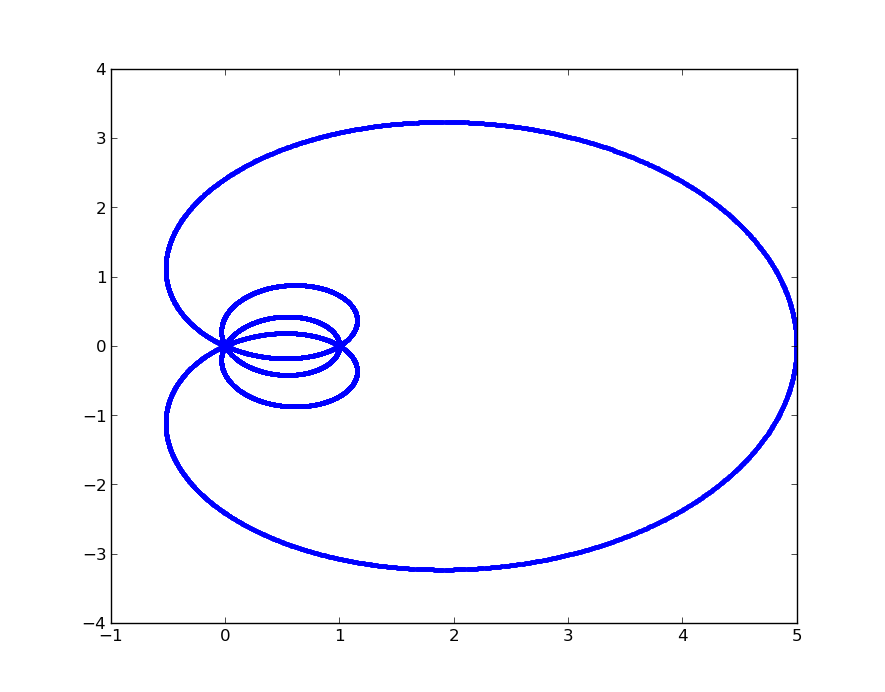
\includegraphics[width=0.8\textwidth]{zn5.png}
    \caption{$n=5$}
\end{figure}

Let $z_1 = e^{i\theta_1}$ and $z_2 = e^{i\theta_2}$ and
$\theta_1$, $\theta_2$ are in $[0, 2\pi)$. Suppose that 
$f_{n}(z_1) = f_{n}(z_2)$ and $\theta_1 < \theta_2$. 
First assume that $\sin (m\theta_1 + \frac{1}{2}\theta_1) = 0
= \sin (m\theta_2 + \frac{1}{2}\theta_2)$ and $\theta_1$, $\theta_2$.
Note that $\sin (\frac{\theta_1}{2})$ and $\sim (\frac{\theta_2}{2})$ can
not equal zero at the same time, since $\frac{\theta_1}{2}$ and 
$\frac{\theta_1}{2}$ are in $[0, \pi)$. Then
\begin{align*}
    \theta_1, \theta_2 \in \{\frac{2k\pi}{2m+1} : k = 1, 2, \ldots, 2m\}. 
\end{align*}
And $f_n(z) = 0$.

Now assume that $\sin (m\theta + \frac{1}{2}\theta) \neq 0$.
We have $\theta_2 = \theta_1 + \frac{2k\pi}{m}$ or
$\theta_2 = \theta_1 + \frac{(2k+1)\pi}{m}$.

First assume that $\theta_2 = \theta_1 + \frac{2k\pi}{m}$, we have
\begin{align*}
    \frac{\sin (m\theta_1 + \frac{1}{2}\theta_1)}
       {\sin (\frac{\theta_1}{2})} =
    \frac{\sin (m\theta_2 + \frac{1}{2}\theta_2)}
       {\sin (\frac{\theta_2}{2})}
\end{align*}
implies
\begin{align*}
    \frac{\sin m\theta_1 \cos (\frac{\theta_1}{2})}
    {\sin (\frac{\theta_1}{2})} + \cos m\theta_1  
    =
    \frac{\sin m\theta_2 \cos (\frac{\theta_2}{2})}
    {\sin (\frac{\theta_2}{2})} + \cos m\theta_2 . 
\end{align*}

If $\sin m\theta_1 \neq 0$ then $\cot (\frac{\theta_1}{2}) = 
\cot (\frac{\theta_2}{2})$. This implies that $\theta_1 = \theta_2$. 

Suppose that $\sin m\theta_1 = 0$, we have 
$\sin (\frac{\theta_1}{2}) \neq 0$ and $\sin (\frac{\theta_2}{2}) \neq 0$,
since $\frac{\theta_1}{2}$ and $\frac{\theta_2}{2}$ are in $[0, \pi)$.
This means that $\theta_1$ and $\theta_2$ are in 
\begin{align*}
    \{\frac{k\pi}{m} : k = 1, 2, \ldots, 2m-1 \}.
\end{align*}
And $f_n(z) = \cos^{2} m\theta = 1$.

Now assume that $\theta_2 = \theta_1 + \frac{(2k+1)\pi}{m}$. Then we have
\begin{align*}
    \frac{\sin (m\theta_1 + \frac{1}{2}\theta_1)}
       {\sin (\frac{\theta_1}{2})} =
    -\frac{\sin (m\theta_2 + \frac{1}{2}\theta_2)}
       {\sin (\frac{\theta_2}{2})}.
\end{align*}
This also implies that
\begin{align*}
    \frac{\sin m\theta_1 \cos (\frac{\theta_1}{2})}
    {\sin (\frac{\theta_1}{2})} 
    =
    \frac{\sin m\theta_1 \cos (\frac{\theta_2}{2})}
    {\sin (\frac{\theta_2}{2})}. 
\end{align*}
Argue as above, we have $\theta_1$ and $\theta_2$ are in 
\begin{align*}
    \{\frac{k\pi}{m} : k = 1, 2, \ldots, 2m-1 \}.
\end{align*}
And $f_n(z) = \cos^{2} m\theta = 1$.   

\begin{lemma}
    For any $re^{i\alpha} \in \C$ and any $\varepsilon > 0$, 
   there exists a $N \in \N$ and a $\theta_{m} \in [0, 2\pi)$
   such that
   \begin{align*}
      |\frac{\sin (m\theta_m + \frac{1}{2}\theta_m)}
       {\sin (\frac{\theta_m}{2})} \left (
   \cos (m\theta_m) + i\sin (m\theta_m) \right) - re^{i\alpha}| 
   < \varepsilon
   \end{align*}
   for any $m \geq N$.
\end{lemma}

\begin{proof}
    Assume that $\alpha = \frac{2\pi i p}{q}$, where $(p, q) = 1$ and 
    $q > p$. For any $m > 1$, consider the set
    \begin{align*}
        \{\frac{2\pi i (p + kq)}{qm} : k = 0, 1, \ldots, m-1 \}. 
    \end{align*}
    Let  
    \begin{align*}
        r_{k} = \frac{\sin (\frac{2\pi i p}{q}+ 
        \frac{\pi i (p + kq)}{qm})}
        {\sin (\frac{\theta_m}{2})}
     = \cos (\frac{2\pi i p}{q}) + \sin (\frac{2\pi i p}{q})
     \cot (\frac{\pi i (p + kq)}{qm}).
    \end{align*}
    Now it is not hard to see that there exist a $N \in \N$ such that
    there is a $0 \leq k_m \leq m-1$ such that 
    $|r_{k_m} - r| \leq \varepsilon$ whenever $m > N$. 
\end{proof}




%-----------------------------------------------------------------------------------
%BIBLIOGRAPHY
%-----------------------------------------------------------------------------------

%\bibliographystyle{unsrt}

%\bibliography{sample}

%-----------------------------------------------------------------------------------

\end{document}
